\section{Experiments and Results}
\label{sec:experiments}
%\vspace{-6pt}

We present in this section results comparing the performance of our algorithm
with the algorithms of Carraghan-Pardalos \cite{pardalos}, 
\"{O}sterg\.{a}rd algorithm \cite{ostergard}, and
Konc and Janezik \cite{konc2007improved}. We implemented the algorithm of \cite{pardalos} ourselves. 
For the algorithm of \cite{ostergard},  we used the publicly available {\it cliquer} source code \cite{cliquer}.
For the algorithm of \cite{konc2007improved}, we used the code {\it MaxCliqueDyn} 
(MCQD, available at {\small \url{http://www.sicmm.org/~konc/maxclique/}}). 
Among the variants available in MCQD, we report results on 
MCQD+CS (which uses improved coloring and dynamic sorting),
since it is the best-performing variant.  

The experiments are performed on a Linux workstation running 64-bit Red Hat Enterprise Linux Server release 6.2 with a 2 GHz Intel Xeon E7540 processor. The codes are implemented in C++ and compiled using gcc version 4.4.6 with -O3 optimization.

%\vspace{-10pt}
\subsection{Test Graphs}
%\vspace{-6pt}

\begin{table}[t]
\small
\centering
\caption{Overview of real-world graphs in the testbed and their origins.}
\label{tab:real-graphs}
\begin{tabular}{ll}
{\bf Graph} & {\bf Description} \\ \hline \hline
{\it cond-mat-2003} \cite{Newman06042004} & A collaboration network of scientists posting preprints 
on \\ & the condensed matter archive at www.arxiv.org in the period \\ \hline %\\ & between January 1, 1995 and June 30, 2003. \\ \hline
%The largest component of this network, which contains 27519 scientists, has been used by several authors as a test-bed for community-finding algorithms for large networks; see for example \cite{PhysRevE.72.027104}
{\it email-Enron} \cite{Leskovec:2005:GOT:1081870.1081893} & A communication network representing
email exchanges. \\
%This data was originally made public, and posted to the web, by the Federal Energy Regulatory Commission during its investigation. 
\hline %Nodes are email addresses and there is a directed edge from \\ & node $i$ to node $j$ if at least one email is sent from $i$ to $j$. \\ \hline
%(In our experiments we ignore the directions and treat the graph as if it were undirected.)\\
%sent at least one email to address $j$, the graph contains a directed edge from $i$ to $j$. Note that non-Enron email addresses act as sinks and sources in the network as we only observe their communication with the Enron email addresses. 
{\it dictionary28} \cite{pajek2006} & Pajek network of words. \\ \hline
{\it Fault\_639} \cite{Ferronato20083922} & A structural problem discretizing a faulted gas reservoir with \\
& tetrahedral Finite Elements and triangular Interface Elements. \\ \hline
%& The Interface Elements are used with a Penalty formulation to simulate fault behavior. \\ \hline
%The problem arises from a 3D discretization with three displacement unknowns associated to each node of the grid. \\
{\it audikw\_1} \cite{Davis97theuniversity} & An automotive crankshaft model of TETRA elements. \\ \hline
{\it bone010} \cite{vanRietbergen199569} &
%Three-dimensional serial reconstruction techniques allow us to develop 
A detailed micro-finite element model of bones representing \\
& the porous bone micro-architecture. \\ \hline
%& Micro computed tomography (CT) is employed to make 3D high-resolution images. \\ \hline
% ($\sim$50 microns) of a bone. \\ \hline
%\\
%Then the 3D reconstruction is directly transformed into an equally shaped micro finite element model by simply converting all bone voxels to equally sized 8-node brick elements. This results in finite element (FE) models with a very large number of elements. \\
{\it af\_shell} \cite{Davis97theuniversity}  & A sheet metal forming simulation network. \\ \hline
{\it as-Skitter} \cite{Leskovec:2005:GOT:1081870.1081893} & An Internet topology graph from trace routes run daily in 2005. \\ \hline %From several scattered sources to million destinations. %1.7 million nodes, 11 million edges. 
{\it roadNet-CA} \cite{Leskovec:2005:GOT:1081870.1081893} & A road network of California.
Nodes represent intersections \\ & and endpoints and edges represent the roads connecting them. \\ \hline % \\ & intersections or endpoints. \\    \hline
{\it kkt\_power} \cite{Davis97theuniversity} & An Optimal Power Flow (nonlinear optimization) network. \\\hline
\end{tabular}
\end{table}

Our testbed is grouped in three categories.

%\vspace{-8pt}
\paragraph{1. Real-world graphs} 
Under this category, we consider 10 graphs (downloaded from the 
University of Florida Sparse Matrix Collection  \cite{Davis97theuniversity}) that originate
from various real-world applications. Table~\ref{tab:real-graphs} gives a quick overview of the graphs and their origins.
  
%\vspace{-8pt} 
\paragraph{2. Synthetic Graphs} 
In this category we consider 15 graphs generated using 
the R-MAT algorithm \cite{Chakrabarti:2006:GML:1132952.1132954}. The graphs
are subdivided in three categories depending on the structures they represent.
\newline {\bf A. Random graphs} (5 graphs) -- Erd\H{o}s-R\'{e}nyi random  graphs generated using R-MAT 
with the parameters (0.25, 0.25, 0.25, 0.25).  Denoted with prefix {\it rmat\_er}.
\newline {\bf B.  Skewed Degree, Type 1 graphs} (5 graphs) -- graphs generated using R-MAT with the parameters (0.45, 0.15, 0.15, 0.25). Denoted with prefix {\it rmat\_sd1}.
\newline {\bf C. Skewed Degree, Type 2 graphs} (5 graphs) --  graphs generated using R-MAT with the parameters (0.55, 0.15, 0.15, 0.15). Denoted with prefix {\it rmat\_sd2}.

%\vspace{-8pt}
\paragraph{3. DIMACS graphs} 
This last category consists of 5 graphs selected from the Second DIMACS Implementation Challenge \cite{dimacs}. 

The DIMACS graphs  are an established benchmark for the maximum
clique problem, but they are of rather limited size and variation. 
In contrast, the real-work networks included  in category 1 of the testset
and the synthetic (RMAT) graphs in category 2
represent a wide spectrum of large graphs posing varying degrees of difficulty for testing the algorithms. 
The {\it rmat\_er} graphs have {\it normal} degree distribution, whereas the {\it rmat\_sd1} and {\it rmat\_sd2} graphs have skewed degree distributions and contain many dense local subgraphs.
 The {\it rmat\_sd1} and {\it rmat\_sd2} graphs differ primarily in the magnitude of maximum vertex degree they contain; the {\it rmat\_sd2} graphs have much higher maximum degree. 
Table \ref{tab:struc-graphs} lists basic structural information (the number of vertices, 
number of edges and the maximum degree) about all 30 of the test graphs.

\begin{table}[t]
\small
%\scriptsize
\centering
\caption{Structural properties---the number of vertices $|V|$; the umber of edges $|E|$; and the maximum degree $\Delta$---of the graphs $G$ in the testbed.
The first ten graphs are the graphs from the UF collection; the next fifteen are the   
RMAT graphs; and the last five are the DIMACS Challenge graphs.}  
\label{tab:struc-graphs}
%\begin{tabular}{l@{\hspace{2pt}}r@{\hspace{5pt}}r@{\hspace{5pt}}r@{\hspace{8pt}}r@{\hspace{5pt}}|@{\hspace{5pt}}l@{\hspace{2pt}}r@{\hspace{5pt}}r@{\hspace{5pt}}r@{\hspace{8pt}}r}
\begin{tabular}{l@{\hspace{5pt}}r@{\hspace{5pt}}r@{\hspace{5pt}}r@{\hspace{5pt}}|@{\hspace{5pt}}l@{\hspace{5pt}}r@{\hspace{5pt}}r@{\hspace{5pt}}r}

\toprule\toprule

$G$ & $|V|$ & $|E|$ & $\Delta$ & $G$ & $|V|$ & $|E|$ & $\Delta$ \\ \hline \hline
{\it cond-mat-2003} & 31,163	& 120,029	 & 202 &	{\it rmat\_sd1\_1} &    131,072 &    1,046,384 & 407           \\ \vspace*{\rowspace}
{\it email-Enron} & 36,692	 & 183,831 &	1,383  &	{\it rmat\_sd1\_2} &    262,144 &    2,093,552 &   558    \\ \vspace*{\rowspace}
{\it dictionary28} & 	52,652 &	89,038 &	38  &		{\it rmat\_sd1\_3} &    524,288 &    4,190,376 &    618  \\ \vspace*{\rowspace}
{\it Fault\_639} &    638,802 &    13,987,881 &    317 &  {\it rmat\_sd1\_4} &    1,048,576 &    8,382,821 &  802    \\ \vspace*{\rowspace}
{\it audikw\_1} &    943,695 &    38,354,076 &    344  &	 {\it rmat\_sd1\_5} &    2,097,152 &    16,767,728 &    1,069   \\

%\midrule
\vspace*{\rowspace}

 {\it bone010} &    986,703 &    35,339,811 &    80 & 
{\it rmat\_sd2\_1} &    131,072 &    1,032,634 &    2,980        \\ \vspace*{\rowspace}
{\it af\_shell10} &    1,508,065 &    25,582,130 &    34 &  
{\it rmat\_sd2\_2} &    262,144 &    2,067,860 &    4,493      \\ \vspace*{\rowspace}
{\it as-Skitter} &    1,696,415 &    11,095,298 &  35,455 &
{\it rmat\_sd2\_3} &    524,288 &    4,153,043 &    6,342     \\ \vspace*{\rowspace}
{\it roadNet-CA} &    1,971,281 &    2,766,607 &    12 & 
{\it rmat\_sd2\_4} &    1,048,576 &    8,318,004 &    9,453      \\ \vspace*{\rowspace}	
{\it kkt\_power} &    2,063,494 &    6,482,320 &    95  &   
{\it rmat\_sd2\_5} &    2,097,152 &    16,645,183 &    14,066    \\

%\midrule
\vspace*{\rowspace}


{\it rmat\_er\_1} &    131,072 &    1,048,515 &    82  &   
{\it hamming6-4} & 64 &    704 &    22 	 \\ \vspace*{\rowspace}
{\it rmat\_er\_2} &    262,144 &    2,097,104 &    98 &  
{\it johnson8-4-4} & 70 &    1,855 &    53   \\ \vspace*{\rowspace} 
{\it rmat\_er\_3} &    524,288 &    4,194,254 &    94  &  
{\it keller4} &    171 &    9,435 &    124  \\ \vspace*{\rowspace}   
{\it rmat\_er\_4} &    1,048,576 &    8,388,540 &    97  & 
{\it c-fat200-5} &    200 &    8,473 &    86  \\ \vspace*{\rowspace} 
{\it rmat\_er\_5} &    2,097,152 &    16,777,139 &    102 & 
{\it brock200\_2} &    200 &    9,876 &    114 \\


\bottomrule\bottomrule
\end{tabular}
%\vspace{-6pt}
\end{table}


%\vspace{-14pt}
\subsection{Results}
%\vspace{-6pt}

\label{sec:exp-results}
%\input{results_timings_new.tex}

\begin{table}[!hbt]

\footnotesize
\scriptsize
%\small
\centering
\caption{Comparison of runtimes (in seconds) of algorithms \cite{pardalos} ({\it CP}),
\cite{ostergard} ({\it cliquer}), \cite{konc2007improved} ({\it MCQD+CS})
and our new exact algorithm ($\tau_{A1}$) for the graphs in the testbed. 
 Columns $P1$, $P2$, $P3$ and $P5$ list the number of vertices/branches pruned in steps Pruning 1, 2, 3 and 5 of our exact algorithm (K stands for $10^3$, M for $10^6$ and B for $10^9$). 
The column $\omega$ (second column) lists the maximum clique size in each graph, 
the column $\omega_{A2}$ lists the clique size returned by our heuristic and the column
$\tau_{A2}$ lists the heuristic's runtime.}
\label{tab:timings}
\begin{tabular}{l@{\hspace{6pt}}r@{\hspace{6pt}}|@{\hspace{6pt}}r@{\hspace{6pt}}r@{\hspace{6pt}}r@{\hspace{6pt}}r@{\hspace{6pt}}|@{\hspace{4pt}}r@{\hspace{4pt}}r@{\hspace{4pt}}r@{\hspace{4pt}}r@{\hspace{4pt}}|@{\hspace{6pt}}r@{\hspace{6pt}}r}

\toprule\toprule
           &  & & &  $\tau_{MCQD}$ & &	&	&	&	&& \\
Graph           	& $\omega$ & $\tau_{CP}$    & $\tau_{cliquer}$  & $_{+CS}$  &  $\tau_{A1}$		& 	$P1$ 		&	$P2$		& 	$P3$ 		&	$P5$		 & $\omega_{A2}$ &  $\tau_{A2}$ \\
\hline \hline
%Graph 			& $\omega$ & $\tau_{CP}$ 	& $\tau_{cliquer}$	& $\tau_{MCQD+CS}$	& $\tau_{new-exact}$ & $\omega_{new-heuristic}$& $\tau_{new-heuristic}$\\ \hline \hline
%\vspace{-4pt} \\
%				& 		& 		 		& 				& $_{-exact}$ 	 	& $_{-heuristic}$ 	& $_{-heuristic}$	\\ \hline \hline
{\it cond-mat-2003} 	& 	25 	& 	4.875 		&  	11.17		&	2.41		&	{\bf 0.011}		& 	29K 			&	48K			&	6,527 		& 	17K			&	25 		& 	$<$0.01 	\\
{\it email-Enron} 	& 	20 	& 	7.005		& 	15.08 		&	3.70		& 	{\bf 0.998}		& 	32K 			&	155K		&	4,060 		& 	8M			&	18 		& 	0.261	\\ %8,835,739	
{\it dictionary28} 	& 	26 	& 	7.700 		&	32.74 		&	7.69		&	{\bf $<$0.01}	& 	52K			& 	4,353		&	2,114		& 	107			&	26 		&	$<$0.01	\\	
{\it Fault\_639}		&	18	&	14571.20		&	4437.14		&	-		&	{\bf 20.03}		&	36			&	13M			&	126			&	1,116		&	18		&	5.80 		\\
{\it audikw\_1}		&	36	&	*			&	9282.49		&	-		&	{\bf 190.17}	&	4,101		&	38M			&	59K			&	721K		&	36		&	58.38 	\\
{\it bone010}		&	24	&	*			&	10002.67		&	-		&	{\bf 393.11}	&	37K			&	34M			&	361K		&	44M			&	24		&	24.39 	\\ %43,991,787
{\it af\_shell10}		&	15	&	*			&	21669.96		&	-		&	{\bf 50.99}		&	19			&	25M			&	75			&	2,105		&	15		&	10.67 	\\
{\it as-Skitter}		&	67	&	24385.73		&	*			&	-		&	{\bf 3838.36}	&	1M			&	6M			&	981K		&	737M		&	66		&	27.08 	\\ %1,656,570	737,899,486
{\it roadNet-CA}	&	4	&	*			&	*			&	-		&	{\bf 0.44}		&	1M			&	1M			&	370K		&	4,302		&	4		&	0.08 		\\ %1,487,640
{\it kkt\_power}		&	11	&	*			&	*			&	-		&	{\bf 2.26}		&	1M			&	4M			&	401K		&	2M			&	11		&	1.83 		\\ %1,166,311	 1,978,595
\midrule
{\it rmat\_er\_1}		&	3	&	256.37		&	215.18		&	49.79	&	{\bf 0.38}		&	780			&	1M			&	915			&	8,722		&	3		&	0.12 		\\
{\it rmat\_er\_2}		&	3	&	1016.70		&	865.18		&	-		&	{\bf 0.78}		&	2,019		&	2M			&	2,351		&	23K			&	3		&	0.24 		\\
{\it rmat\_er\_3}		&	3	&	4117.35		&	3456.39		&	-		&	{\bf 1.87}		&	4,349		&	4M			&	4,960		&	50K			&	3		&	0.49 		\\
{\it rmat\_er\_4}		&	3	&	16419.80		&	13894.52		&	-		&	{\bf 4.16}		&	9,032		&	8M			&	10K			&	106K		&	3		&	1.44 		\\
{\it rmat\_er\_5}		&	3	&	*			&	*			&	-		&	{\bf 9.87}		&	18K			&	16M			&	20K			&	212K		&	3		&	2.57 		\\
%\midrule
{\it rmat\_sd1\_1}	&	6	&	225.93		&	214.99		&	50.08	&	{\bf 1.39}		&	39K			&	1M			&	23K			&	542K		&	6		&	0.45 		\\
{\it rmat\_sd1\_2}	&	6	&	912.44		&	858.80		&	-		&	{\bf 3.79}		&	90K			&	2M			&	56K			&	1M			&	6		&	0.98 		\\ %1,399,314	
{\it rmat\_sd1\_3}	&	6	&	3676.14		&	3446.02		&	-		&	{\bf 8.17}		&	176K		&	4M			&	106K		&	2M			&	6		&	1.78 		\\ %2,677,437
{\it rmat\_sd1\_4}	&	6	&	14650.40		&	13923.93		&	-		&	{\bf 25.61}		&	369K		&	8M			&	214K		&	5M			&	6		&	4.05 		\\ %5,566,602
{\it rmat\_sd1\_5}	&	6	&	*			&	*			&	-		&	{\bf 46.89}		&	777K		&	16M			&	455K		&	12M			&	6		&	9.39 		\\ %12,168,698
%\midrule
{\it rmat\_sd2\_1}	&	26	&	427.41		&	213.23		&	{\bf 48.17}	&	242.20		&	110K		&	853K		&	88K			&	614M		&	26		&	32.83 	\\ %614,813,037
{\it rmat\_sd2\_2}	&	35	&	4663.62		&	{\bf 851.84}	&	-		&	3936.55		&	232K		&	1M			&	195K		&	1B			&	35		&	95.89 	\\ %1,044,068,886
{\it rmat\_sd2\_3}	&	39	&	13626.23		&	{\bf 3411.14}	&	-		&	10647.84		&	470K		&	3M			&	405K		&	1B			&	37		&	245.51 	\\ %1,343,563,239
{\it rmat\_sd2\_4}	&	43	&	*			&	{\bf 13709.52}	&	-		&	*			&	*			&	*			&	*			&	*			&	42		&	700.05 	\\
{\it rmat\_sd2\_5}	&	N	&	*			&	*			&	-		&	*			&	*			&	*			&	*			&	*			&	51		&    1983.21 	\\
%\vspace*{\rowspace}
\midrule
{\it hamming6-4}	&	4	&	{\bf $<$0.01}	&	{\bf $<$0.01}	&{\bf $<$0.01}	&	$<$0.01		&	0			&	704			&	0			&	0			&	4		&	$<$0.01 	\\
{\it johnson8-4-4}	&	14	&	0.19			&	{\bf $<$0.01}	&{\bf $<$0.01}	&	0.23			&	0			&	1,855			&	0			&	0			&	14		&	$<$0.01 	\\
{\it keller4}		&	11	&	22.19		&	0.15			&	{\bf 0.02}	&	23.35		&	0			&	9,435			&	0			&	0			&	11		&	$<$0.01 	\\
{\it c-fat200-5}		&	58	&	0.60			&	0.33			&	{\bf 0.01}	&	0.93			&	0			&	8,473			&	0			&	0			&	58		&	0.04 		\\
{\it brock200\_2}	&	12	&	0.98			&	0.02			&{\bf $<$0.01}	&	1.10			&	0			&	9,876			&	0			&	0			&	10		&	$<$0.01 	\\
\bottomrule\bottomrule
\end{tabular}
%\vspace{-6pt}

\end{table}



Table \ref{tab:timings} shows the size of the maximum clique ($\omega$) and the runtimes  of our exact algorithm (Algorithm 1) and the algorithms of Caraghan and Pardalos (CP), 
\"{O}sterg\.{a}rd ({\it cliquer}) 
and Konc and Jane\v{z}i\v{c}  (MCQD+CS) for all the graphs in the testbed. 
The last two columns show the results of our heuristic (Algorithm 2)---the size of the maximum clique 
returned  and its runtime. The columns labeled $P1$, $P2$, $P3$ and $P5$ list the number of 
vertices/branches pruned in the respective pruning steps of Algorithm 1.
Pruning 4 is omitted since it is used by all the algorithms compared in the table. These numbers have been rounded  (K stands for $10^3$, M for $10^6$ and B for $10^9$), although the exact numbers can be found in the Appendix (Table \ref{tab:prunings}).

In Table \ref{tab:timings}, the fastest runtime for each instance is indicated with boldface. 
An asterisk (*) indicates that an algorithm did not terminate within 25,000 seconds for a particular
instance. A hyphen (-) indicates that the publicly available implementation 
(the {\it MaxCliqueDyn} code) had to be aborted because the input graph was too large 
for the implementation to handle. Even for the instances for which the code
eventually run successfully, we had to first modify 
the graph reader to make it able to handle graphs with multiple connected components.
For the graph {\it rmat\_sd2\_5}, none of the algorithms computed the maximum clique size in 
a reasonable time; the entry there is marked with N, standing for  ``Not Known''.

We discuss in what follows our observations from this table
for the exact algorithm and the heuristic.

%\vspace{-10pt}
\subsubsection{Exact algorithms}
\label{sec:exp-exact}

As expected, our exact algorithm gave the same size of maximum clique as the other
three algorithms for all test cases. 
In terms of runtime,  its relative performance compared to the other three varied
in accordance with the advantages afforded by the various pruning steps.  


\begin{figure}
  \centering
    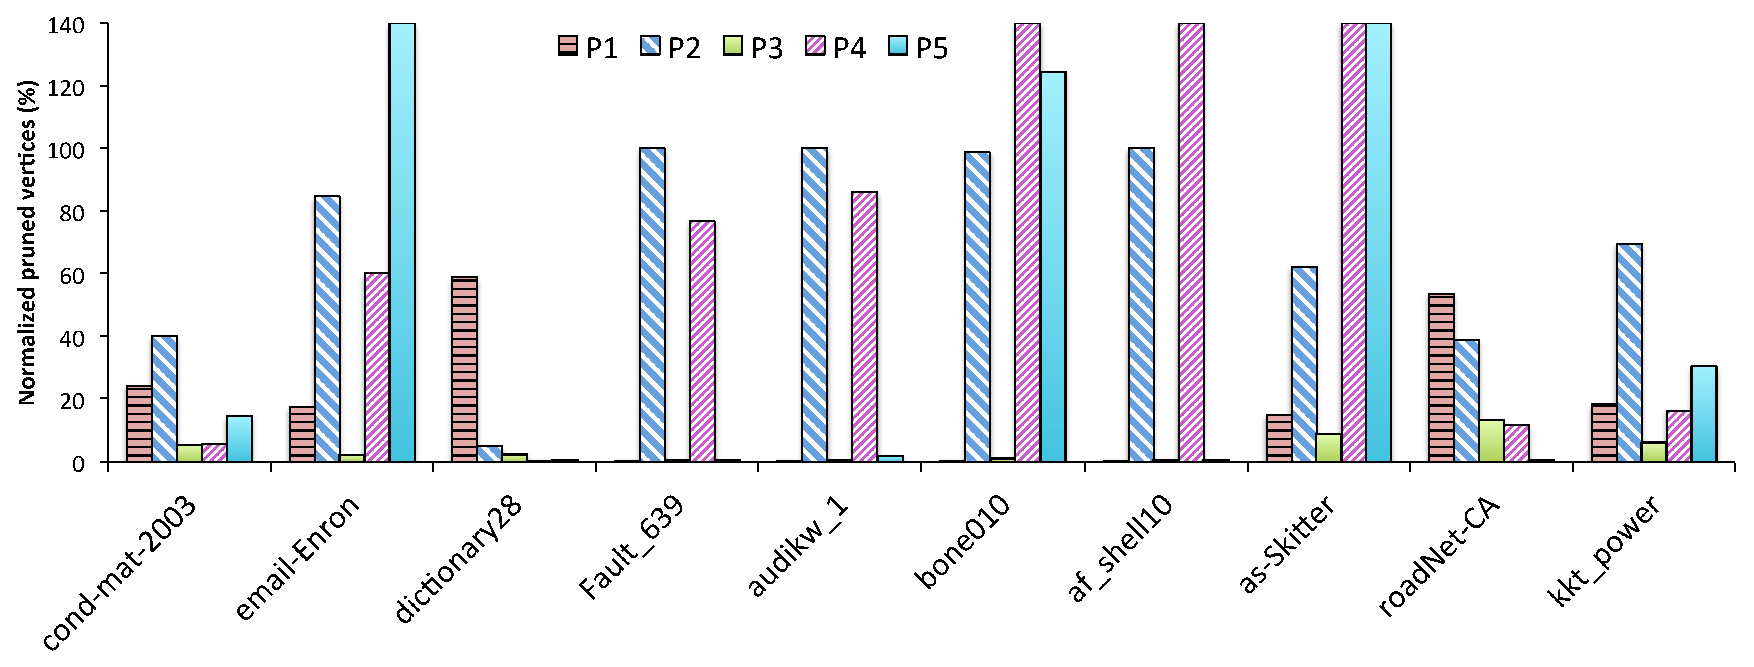
\includegraphics[scale=0.4]{pruned.eps}
\caption{Number of ``pruned" vertices in the various pruning steps normalized
by the number of edges in the graph (in percents) for the test graphs in category 1 (we cut few bars reachining 140\% as their correspnding values are much higher).}
\label{fig-pruningplot}
\end{figure}

%{\bf Analysis of pruning steps.  }
Vertices that are discarded by Pruning 1 are skipped in the main loop of the algorithm, and the largest cliques containing them are not computed. Pruning 2 avoids re-computing previously computed cliques in the neighborhood of a vertex. In the absence of Pruning 1, the number of vertices pruned by Pruning 2 would be bounded by the number of edges in the graph (note that this is more than the total number of vertices in the graph). While Pruning 3 reduces the size of the input set on which the maximum clique is to be computed, Pruning 5 brings down the time taken to generate the intersection set in Line 12 of the subroutine. 
Pruning 4 corresponds to back tracking. Unlike Pruning steps 1, 2, 3 and 5, Pruning 4
is used  by all three of the other algorithms in our comparison. The primary strength of our algorithm is its ability to take advantage of pruning in multiple steps in a hierarchical fashion, allowing for opportunities for one or more of the steps to kick in and impact performance.

In Figure~\ref{fig-pruningplot} we show the number of vertices discarded by all
the  pruning steps of the exact algorithm normalized by the total number of edges
in a graph for the real-world graphs (category 1) in the testbed. We cut few bars reachining
140\% as their correspnding values are much higher.
The Appendix, we provide a complete tabulation of the raw numbers for the pruned vertices in all the steps for all the graphs in the testbed. It can be seen for these graphs pruning steps 2 and 5 in particular discard a large percentage of vertices, potentially resulting in large runtime savings. The general behavior of the pruning steps Pruning 1, 2, 3 and 5 for the synthetic graphs {\em rmat\_er} and {\em rmat\_sd1} was observed to be somewhat similar to that depicted in Figure~\ref{fig-pruningplot} for the real-world graphs. In contrast, for the DIMACS graphs, the number of vertices pruned in steps Pruning 1, 3 and 5 were observed to be zero; the numbers in the step Pruning 2 were nonzero, but relatively modest.
%Since our new pruning steps hierarchically reduce the search space, one can expect a decreasing order of effect in the performance of Prunings 1, 2, 3 and 5, with Pruning 1 having the highest impact, and 5 the lowest. 

As a result  of the differences seen in the effects of the pruning steps, as discussed below,
the runtime performance of our algorithm (seen in Table \ref{tab:timings}) compared
to the other three algorithms varied in accordance with the difference in the structures represented 
by the different categories of graphs in the testbed.

{\bf Real-world Graphs. }
For most of the graphs in this category, it can be seen that our algorithm runs several orders of magnitude faster than the other three, mainly due to the large amount of pruning the algorithm enforced. These numbers also illustrate the great benefit of hierarchical pruning. 
For the graphs {\em Fault\_639}, {\em audikw\_1} and {\em af\_shell10}, 
there is only minimal impact by Prunings 1, 3 and 5,
whereas Pruning 2 makes a big difference resulting in impressive runtimes. 
The number of vertices pruned in steps Pruning 1 and 3 varied among the 
graph {\em within} the
category, ranging from 0.001\% for {\it af\_shell} to a staggering 97\% for {\it as-Skitter} 
for the step Pruning 1. 
%We observe that the relative speedup factor of our algorithm is the highest for
%the graphs with high maximum clique size and high maximum degree.
%as well. For instance, for as-Skitter reduction the search space is reduced dramatically due to pruning, and results in a very impressive performance.


{\bf Synthetic Graphs. }
For the synthetic graph types {\it rmat\_er} and {\it rmat\_sd1}, our algorithm clearly outperforms 
the other three by a few orders of magnitude in all cases. 
This is also primary due to the high number of vertices discarded by the new pruning steps. 
In particular, for {\it rmat\_sd1} graphs, between 30 to 37\% of the vertices are pruned just in the step Pruning 1. 
%The {\it rmat\_er} and the corresponding {\it rmat\_sd1} graphs have nearly equal number of vertices and edges, however, the timings of the {\it rmat\_er} graphs are relatively better because of the smaller size of the maximum clique and the smaller maximum degree. 
For the {\it rmat\_sd2} graphs, which have relatively larger maximum clique and higher maximum degree than the {\it rmat\_sd1} graphs, our algorithm is observed to be faster than 
CP but slower than {\em cliquer}. 

{\bf DIMACS Graphs. }
The runtime of our exact algorithm for the DIMACS graphs is 
in most cases comparable to that of CP and higher than that of {\it cliquer}
and {\it MCQD+CS}.
%As can be seen from the Table  \ref{tab:timings}, 
For these graphs, only Pruning 2 was found to be effective, 
and thus the performance results agree with one's expectation. 
%We include in the Appendix timing results on a larger collection of DIMACS graphs. 

It is to be noted that the DIMACS graphs are intended to serve as challenging test cases for the maximum clique problem, and graphs with such high edge densities and low vertex count are rare in practice. 
Most of these have between 20 to 1024 vertices with an average edge density of roughly 0.6, 
whereas, most real world graphs are often very large and sparse. Good examples are Internet topology graphs \cite{Faloutsos:1999:PRI:316188.316229}, the web graph \cite{kumar:extracting}, social network graphs \cite{Domingos:2001:MNV:502512.502525}, and the real-world graphs in our testbed. 

%\vspace{-15pt}
\subsubsection{The Heuristic}
\label{sec:exp-heuristic}

It can be seen that our heuristic runs several orders of magnitude faster than our exact algorithm,
while delivering either optimal or very close to optimal solution.
It gave the optimal solution on 25 out of the 30 test cases.
On the remaining 5 cases where it was suboptimal, its accuracy ranges from 83\% to 99\% (on average 93\%).
Additionally, we run the heuristic by choosing a vertex randomly in Line \ref{maxDsel} of Algorithm \ref{alg:mClqHeu} instead of the one with the maximum degree. We observe that on average, the solution is optimal only for less than $40\%$ of the test cases compared to 83\% when selecting the maximum degree vertex.
%after three repetitions with different random seeds

Figure~\ref{fig-timeplot} provides an aggregated visual summary of the runtime trends of
the various algorithms across the five categories of graphs in the testbed. 
%The bars in each category
%are created as follows. First the runtime for each algorithm for each graph in a category is divided by the runtime of the slowest algorithm for that graph. Then the mean of these is taken as a resut for the category. Values enter into the mean calculation when runtimes are available for
%at least three algorithms.

%\vspace{-10pt}
%\vspace{-10pt}
\begin{SCfigure}
  \centering
    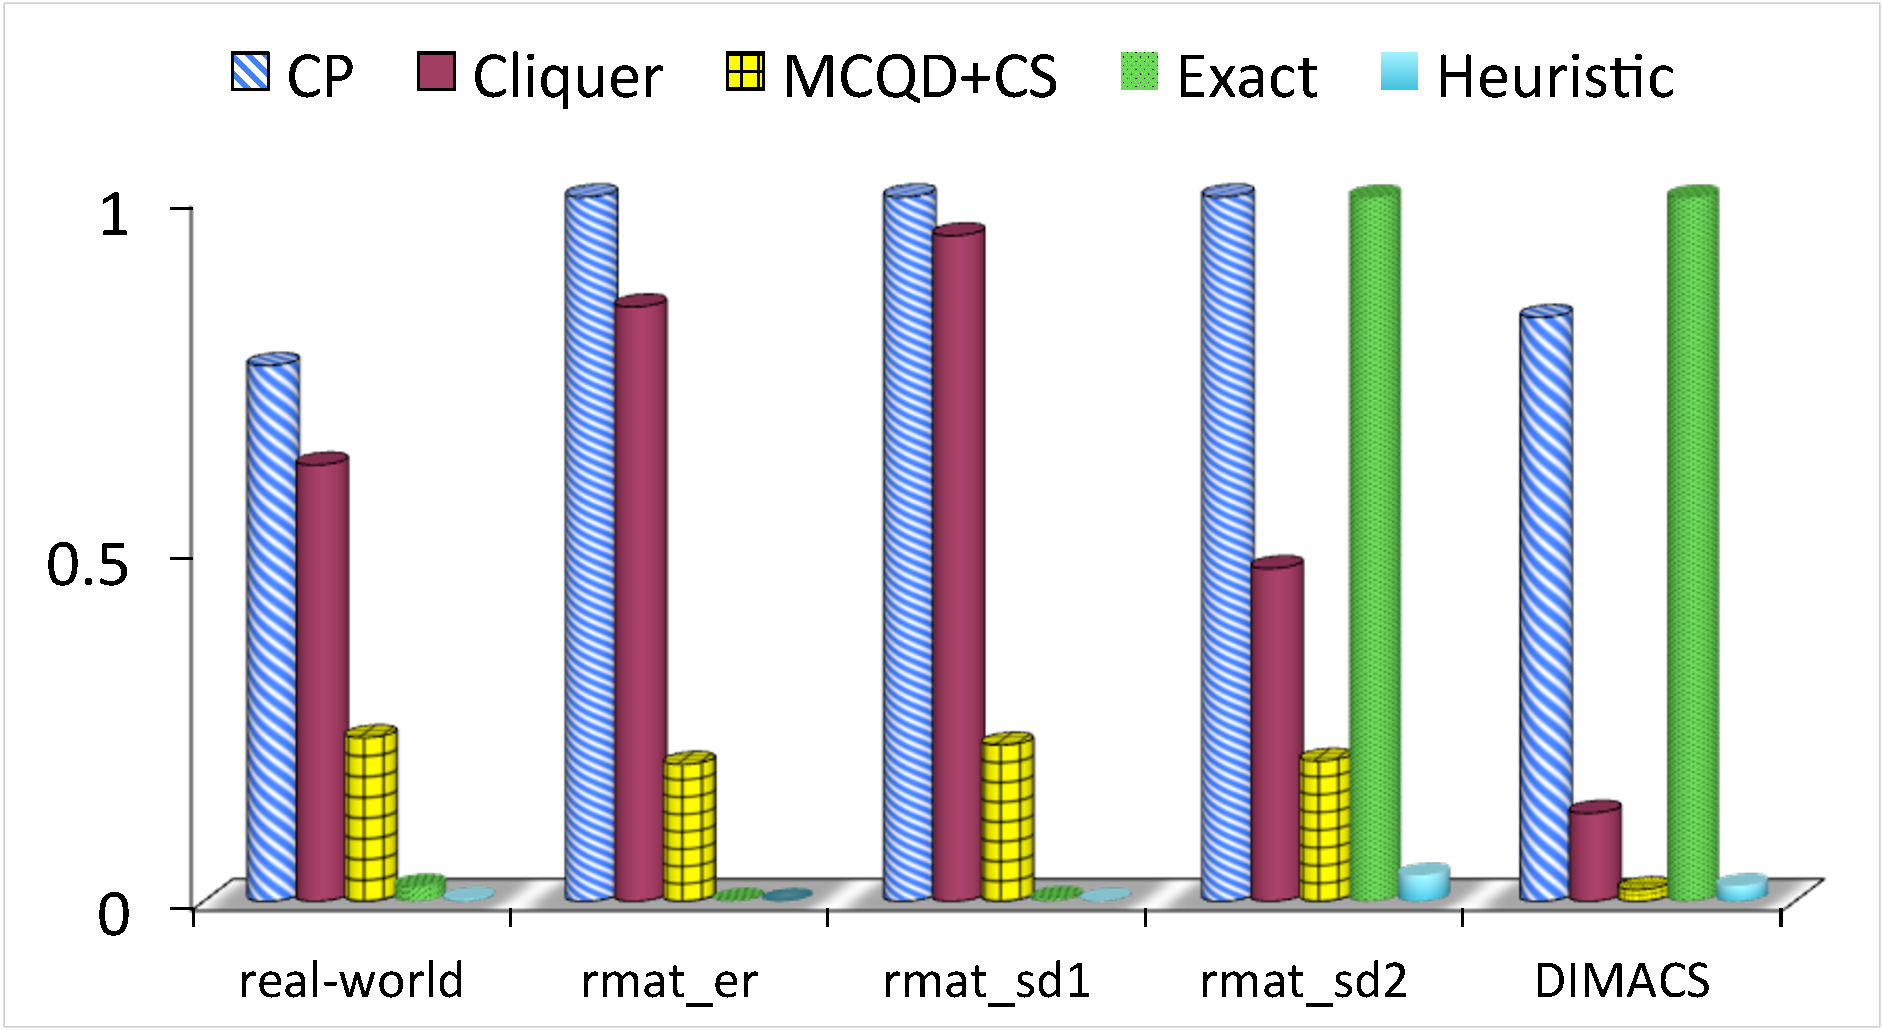
\includegraphics[width=7.0cm]{maxclqplot.eps}
%%\vspace{-30pt}
  \caption{Runtime (normalized, mean) comparison between various algorithms. For each category of graph, first, all runtimes for each graph were normalized by the runtime of the slowest algorithm for that graph, and then the mean was calculated for each algorithm. Graphs were considered only if the runtimes for at least three algorithms was less than the 25,000 seconds limit set.}
\label{fig-timeplot}
\end{SCfigure}
%\vspace{-10pt}
%\vspace{-10pt}


To give a sense of runtime growth rates, we provide in Figure~\ref{fig-runtimeplots} plots of the 
runtime of the new exact algorithm and the heuristic for the synthetic and real-world graphs 
in the testbed. Besides the curves corresponding to the runtimes of the
{\em exact} algorithm and the {\em heuristic}, the figures also include a curve corresponding to
the number of {\em edges} in the graph divided by the clock frequency of the computing
platform used in the experiment. This curve is added to facilitate comparison between
the growth rate of the algorithms with that of a linear-time (in the size of the graph) growth rate. 
It can be seen that the runtime of the heuristic by and large grows 
somewhat linearly with the size of a graph. The exact algorithm's runtime, which is orders of
magnitude larger than the heuristic, exhibited a similar growth behavior for these test-cases
(even though its worst-case complexity suggests exponential growth). 

\begin{figure}
  \centering
    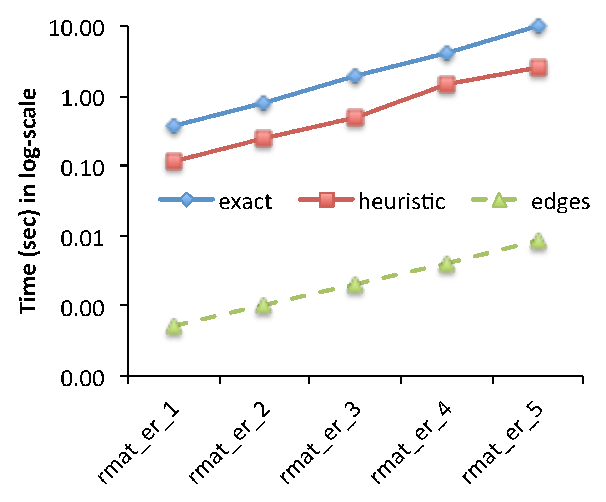
\includegraphics[scale=0.6]{compare_time_er.eps}
    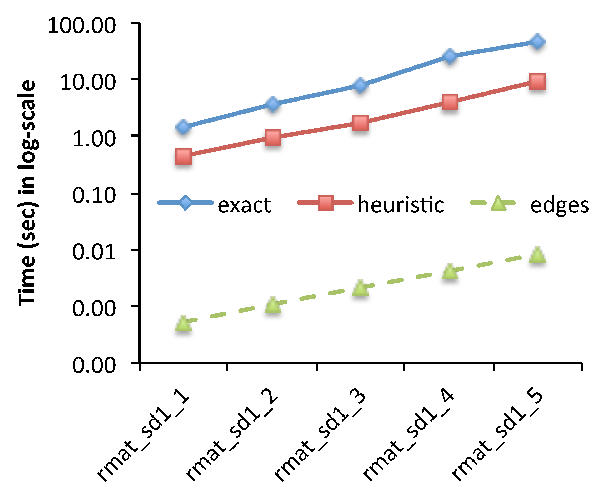
\includegraphics[scale=0.6]{compare_time_sd1.eps}
    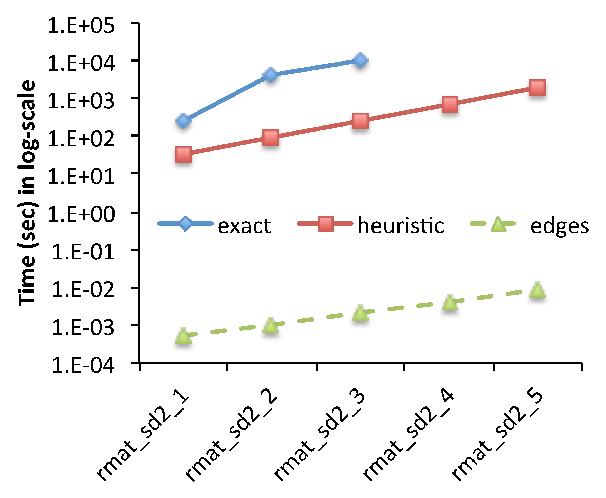
\includegraphics[scale=0.6]{compare_time_sd2.eps}
    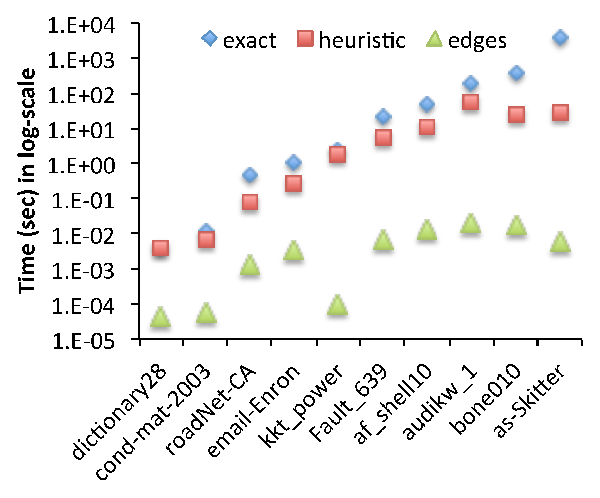
\includegraphics[scale=0.6]{compare_time_rw.eps}
    
%%\vspace{-30pt}
 \caption{Run time plots of the new exact and heuristic algorithms. The third curve, labeled
 {\em edges}, shows the quantity, number of edges in the graph divided by the clock 
 frequency of the computing platform used in the experiment. 
 }
\label{fig-runtimeplots}
\end{figure}


%Finally, we comment on our experience in using the 
%{\it MaxCliqueDyn} code.
%Unfortunately, the code failed to execute most of the  
%large instances in our testbed, including the majority of the RMAT and real-world instances,
%due to memory management issues in the code. 
%The entries in Table~\ref{tab:timings} marked with hyphen (-) show instances
%for which the code crashed.
%One of the few instance we were able to successfully run was {\it email-enron}.
%For it, the code took 4.91 seconds to compute the maximum clique 
%(using the same experimental setup), whereas our algorithm took only 0.998 seconds. 
%The memory issue also prevented us from do an extensive comparison with the other more recent algorithms 
%based on \cite{citeulike:7905505} and including \cite{Tomita:2007:EBA:1188122.1188130}, 
%since to our knowledge, there does not exist any other publicly available package 
%based on this algorithm. 
%On a related note, our attempts to run instances larger than the ones used in the experiments reported here on the
%the {\em cliquer}  package (\url{http://users.tkk.fi/pat/cliquer.html} \cite{cliquer}) failed because of similar memory leak issues. 
%This makes our code (available at \url{http://cucis.ece.northwestern.edu/projects/MAXCLIQUE/}) the only open source code,
%which has been tested to be capable of finding the maximum clique of large instances. Note that our code also
%includes a converter between two popular graph formats, DIMACS to/from matrix market.
%Even for the instances it eventually run successfully, we had to first make modifications to the graph reader
%to make it able to handle graphs with multiple connected components.
%{\it 
%The fixes and related discussion I had to do in the available source code of MaxCliqueDyn \cite{konc2007improved} is as follows:
%The graph reader fails to read large graphs specially when the graph contains disjoint vertices. 
%The reader tries to allocate memory based on the number of distinct vertices and it 
%assumes the number of vertices is equal to the number of distinct vertices (which could be much lower) as the package
%has mostly been developed keeping the densed small graphs in mind. 
%Because of this there code can't run for the massive sparse graphs as the vertex ID becomes higher
%than the number of vertices and therefore access invalid memory locations and gives segmentation fault.
%I guess the reason they do this is to reduce the required memory by the algorithm (as the reply from the author says,
%at every round it allocates memory equal to the number of vertices, and therefore eventually the expected space requirement
%could be O($n^2$)). We therefore fixed the problem 
%by disallowing the code to change the number of vertices to the number of dictinct vertices.
%After doing this we noticed that the reader is capable of loading larger sparse graphs, but the algorithm runs 
%for long time and incrementally asks huge memory and the job become killed at some point
%For example, we noticed when we run experiment on $Fault$ graph, its being killed when
%the allocated memory reaches 100 GB.
%}

%\subsection{Example of an application in social network analysis}
\label{sec:applications}

We conclude this section on experiments with a small example 
demonstrating the application of the clique algorithms for detecting overlapping communities in social networks. 
In many real networks vertices may belong to more than one group, and such groups form overlapping communities. Classical examples are social networks, where an individual usually belongs to different circles at the same time, from that of work colleagues to family, sport associations, etc. 
Finding overlapping communities is a challenging problem \cite{Fortunato_2010}.
Clique algorithms are one way in which a solution can be found.  
%A detailed overview of community detection methods, and the significance and complexity involved in overlapping community findingcan be found in \cite{Fortunato_2010}.

%\vspace{-20pt}
\begin{figure}%[h!]
  \centering
    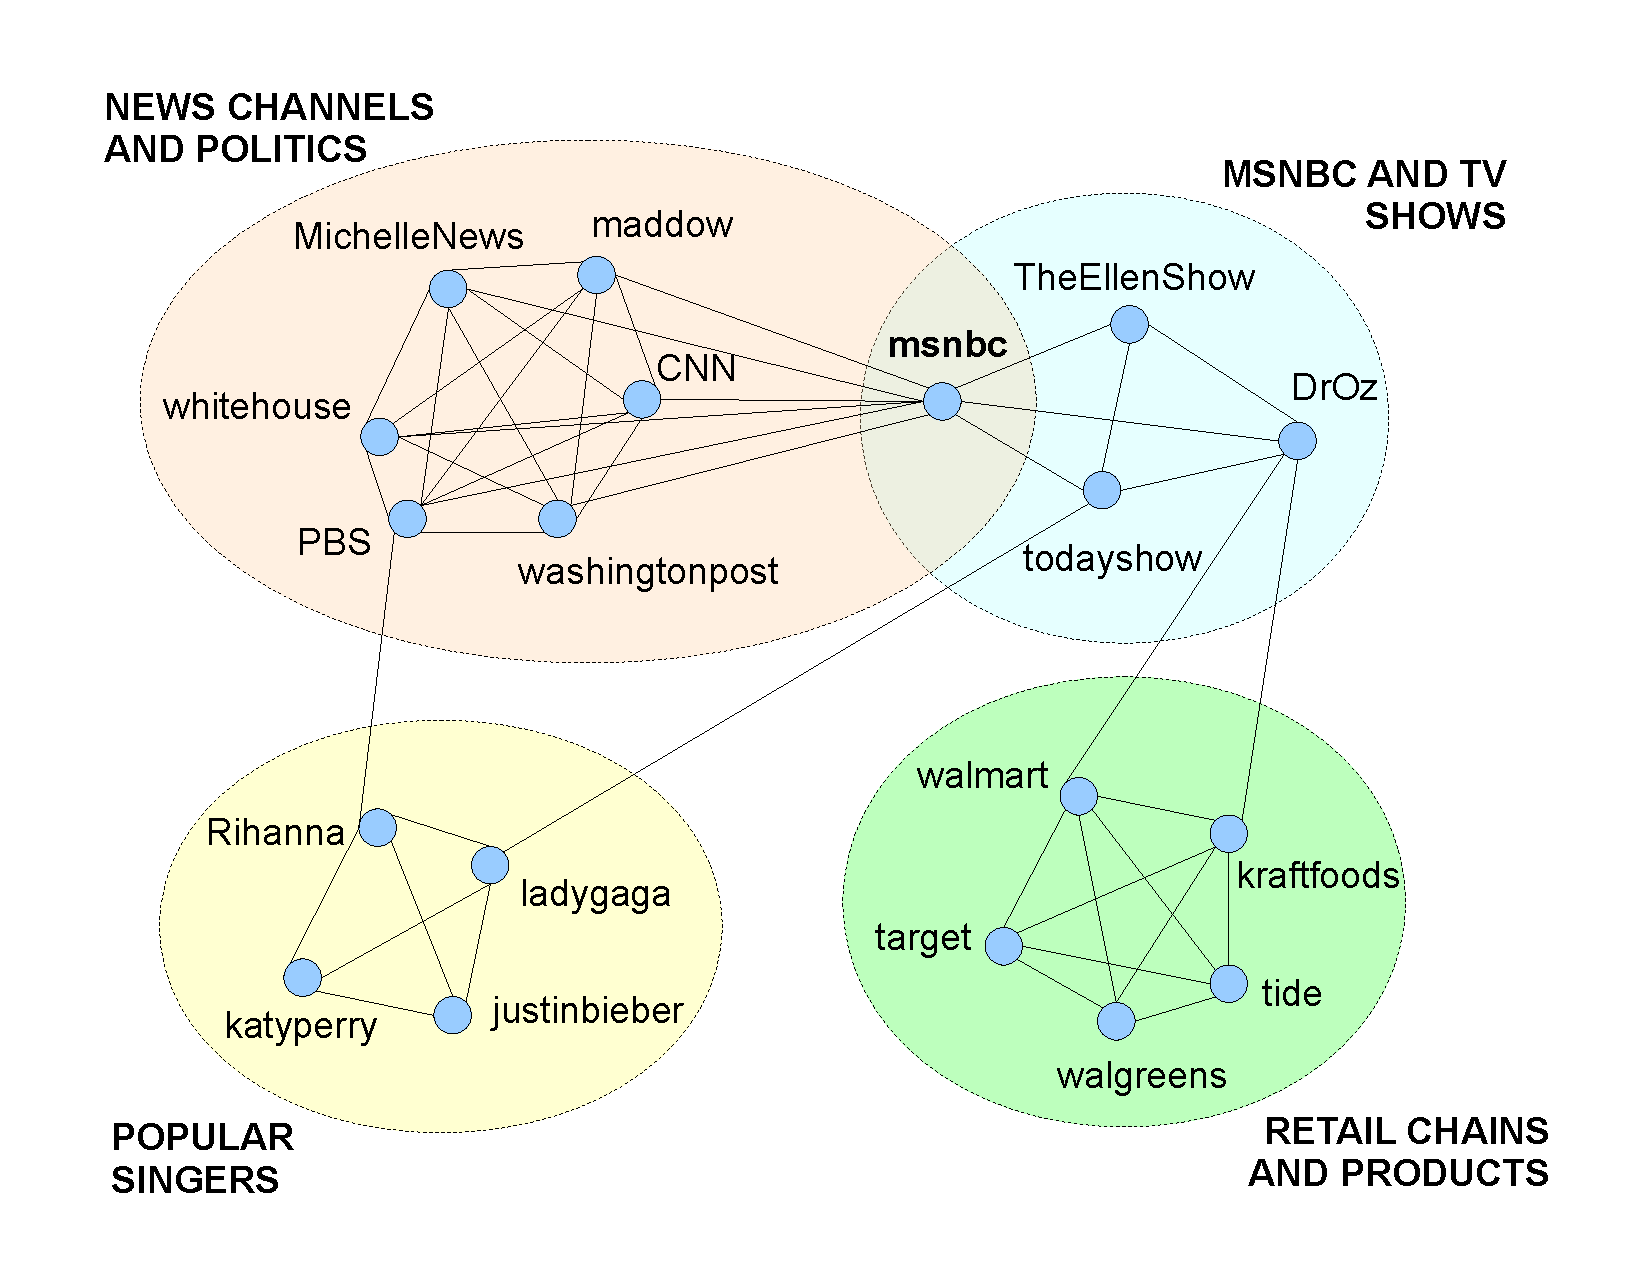
\includegraphics[width=1\textwidth]{communities.pdf}
%\vspace{-30pt}
  \caption{Some Facebook communities detected by our max clique heuristic.}
\label{fig-communities}
\end{figure}
%\vspace{-10pt}

%\footnotetext{http://www.facebook.com}
For our small experiment, we use data collected from Facebook\footnote[1]{http://www.facebook.com}.
Every user on Facebook has a {\it wall}, which is a the user's profile space that allows the posting of messages, often short or temporal notes by other users. The user comments and user information from specific {\it walls} are publicly available and we collected them using Facebook API. We constructed a graph with the {\it walls} as vertices. Any two users who have commented on the same {\it wall} indicate a connection between the {\it walls}, and we form an edge between them. There could be many common users for each wall, and so we assigned edge weights by Jacard index or similarity coefficient \cite{Leydesdorff}. Once this is done for all {\it walls}, we retained only those edges which have weights above a chosen threshold, indicating a strong correlation. The threshold is a user's choice and decides both the size and the number of communities found.
% If an edge already exists, we increase the edge weight by 1. Once this is done for all {\it walls}, the edge weights are normalized, and we retain only those edges which have edge weights above a chosen threshold (we use 0.01), indicating a strong correlation.

%duplicate removal
We modified our heuristic to retain the largest maximum clique containing each node. 
%This is done by simply substituting Lines 3 and 4 of Algorithm \ref{alg:clqHeu}, with a simple routine that stores each clique in a preferred data structure. 
The exact algorithm could have also been used instead of the heuristic for this purpose. We choose the heuristic since it is much faster and for this particular problem of community detection the accuracy of the size of cliques formed is not critical.

Figure \ref{fig-communities} shows some of the cliques/communities detected. We see two isolated communities, one for popular singers, and another for retail chains and products. We also see a community for news channels and politics, and a community of MSNBC and popular TV shows. The highlight of this experiment  is that the
clique algorithm allows a node to be a member of more than one community giving an overlapping community structure. Although the {\it news channels and politics} and {\it MSNBC and tv shows} communities are not directly related and have different members, they share a common member.
%add from nature paper why this is significant. coexistence of their structural subunits 



%\vspace{-10pt}